\Lecture{Jayalal Sarma}{Oct 19, 2020}{18}{Introduction to Ramsey Numbers}{Shivlal Gangesh}{$\alpha$}{JS}
\section{Introduction}
Till now we have seen advanced versions of the discrete mathematics topics we already know. Now we are going to get into Extremal combinatorics. Here we are interested in questions of the form 
\begin{itemize}
\item \textit{If this structure appears, then what is the minimum/maximum size of the object?}
\item \textit{If the size is at least this much , then what kind of structures appear in the object?}
\item \textit{What is the minimum size of the collection such that it is guaranteed to have certain property?}
\end{itemize}
In general we are interested in the extreme behaviors in combinatorics. The classic example we start with is an extension to an example that we have done in the beginning of the course as an Application of Pigeon Hole Principle.
\section{Starting Point} \label{R(3,3)}
\begin{theorem}
Six people meet in a party. Then either there exist three people who are friends with each other or there exist three people who are strangers with each other.(Note : Any two people can either be friends or strangers)
\end{theorem}
We are interested in proving the above statement. Lets look into two different approaches
\subsection{Model 1 (Using Cliques and Independent Sets)}
\begin{description}
   \item[Model] Let us represent the problem as a $6$ vertex graph $G(V,E) $with each person corresponding to a vertex. $(u,v) \in E$ if and only if person $u$ is a friend of person $v$.
In this Model the original statement can be reformulated as
\item[Statement]
\textit{Any graph on $6$ vertices must either have a clique on $3$ vertices or an independent set on $3$ vertices.
\item}
\begin{proof}
 Consider any vertex $v$ in the graph G, without loss of generality we can assume that the degree of $v$ is greater than or equal to $3$  because suppose it is not the case then consider $\overline{G}$ ; as $\textrm{Cliques in }G \leftrightarrow \textrm{Independent Sets in } \overline{G} $.\\
 Let the $3$ neighbours of $v$ be $a$, $b$ and $c$. Consider the two exhaustive cases :
 \begin{description}
    \item[Case 1 : There are no edges among $a$, $b$ and $c$]
    $ $ \newline
    Here we have $\{a, b, c\}$ as the 3-Independent Set
    \item[Case 2 : There is at least one edge among $a$, $b$ and $c$ ]
    $ $ \newline
    Let $(a,b) \in E$ be that edge, then we have $\{v, a, b\}$ as the 3-clique
 \end{description}
Therefore the given statement holds true.
\end{proof}
\item[Proof for tightness]
To prove that this is tight we need to show there is a graph with $5$ vertices such that it does not have 3-clique and 3-Independent Set. Given below is one such  example
\begin{figure}[h!]
    \centering
    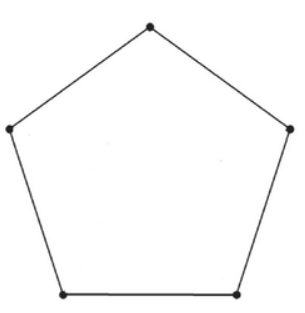
\includegraphics[width=0.2\linewidth]{images/r33counter_example.png}
    \caption{5-vertex graph with no 3-clique and no 3-Independent Set}
\end{figure}
\end{description}
\subsection{Model 2 (Using Graph Edge colouring)}
\begin{description}
   \item[Model]
   Let us represent the problem as 2-edge coloring of a $K_6$ graph with each vertex corresponding to a person. Color the edge $(u,v)$ with \textit{red} if $u$ and $v$ are friends, color it with \textit{blue} if $u$ and $v$ are strangers.
In this Model the original statement can be reformulated as
\item[Statement]
\textit{For any 2-edge colouring of $K_6$, there must exist either  a red $K_3$  or a blue $K_3$ }
\item
\begin{proof}
 Consider any Red,Blue-edge coloring of $K_6$. Consider any vertex $v$, the degree of $v$ is $5$ as the graph is a complete graph. By Pigeon Hole Principle , $v$ must have either $3$ red edges incident on it or $3$ blue edges incident on it. Consider the case when $v$ is incident on with $3$ red edges. Let the 3 neighbours of $v$ be $a$, $b$ and $c$.  Now there are 2 cases :
 \begin{description}
    \item[Case 1 : There is no red colored edge among $(a,b)$, $(b,c)$ and $(c,a)$ ]
    $ $ \newline
    Then all the three edges $(a,b)$, $(b,c)$ and $(c,a)$ are colored blue. Therefore $\{a, b, c\}$ forms a blue $K_3$
    \item[Case 2 : There is at least one red colored edge among $(a,b)$, $(b,c)$ and $(c,a)$ ]
    $ $ \newline
    Let $(a,b)$ be the red colored edge, then $\{v, a, b\}$ forms a red $K_3$
 \end{description}
 Therefore the given statement holds true.
\end{proof}
\item[Proof for tightness]
To prove that this is tight we need to show there is a 2-edge coloring of $K_5$ Such that it does not have red $K_3$ and blue $K_3$. Given below is one such  example
\begin{figure}[h!]
    \centering
    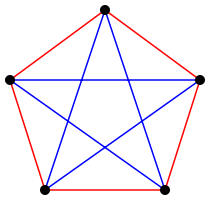
\includegraphics[width=0.2\linewidth]{images/k5counter_example.png}
    \caption{2-edge coloring of $K_5$ with no red $K_3$ and no blue $K_3$}
\end{figure}
\end{description}

Generalizing the above problem with arbitrary red $k_p$ and blue $k_q$ has been extensively studied by Ramsey and has led to the definition of Ramsey numbers.
\section{Ramsey numbers}
\begin{definition}[Ramsey number]
The Ramsey number denoted by $R(p,q)$ is the minimum number of vertices say $n$ such that any 2-edge coloring of $K_n$ must have either a red $K_p$ or a blue $K_q$.\\
(\textbf{Or equivalently as})\\
The minimum number of vertices ($n$) such that any graph on $n$ vertices must either have a clique on $p$ vertices or an independent set on $q$ vertices.
\end{definition}

\subsection{Some Observations}
\begin{property}
$R(3,3)=6$
\end{property}
This is the direct formulation of the example we have done previously in \ref{R(3,3)}
\begin{property}
$R(p,q) = R(q,p)$
\end{property}
The colors \textit{red} and \textit{blue} are just placeholders for two colors, thus swapping the colors will still preserve the Ramsey number property. Therefore $R(p,q) = R(q,p)$.
\begin{property}
$\forall l \geq 1 \quad R(l,1) = 1$
\end{property}
The existence of a blue $K_1$ is nothing but the presence of single vertex and any graph with a single vertex satisfies this property. Therefore $R(l,1) = 1$


\section{Existence of R(p,q)}
The Proof for the existence of $R(p,q)$ is due to Erdős–Szekeres. The existence was proved by providing an upper bound as a recurrence relation as follows :
\begin{theorem}
$$\forall p,q \geq 2 \quad R(p,q) \; \leq \; R(p,q-1) + R(p-1,q) $$
\end{theorem}
\begin{proof}
 Let us prove this by mathematical induction on $n$ where $n=p+q$.
 \begin{description}
    \item[Idea] To show the upper bound for $R(p,q) \leq n$ , we must argue that for any 2-edge coloring of $K_n$ there exist a red $K_p$ or blue $K_q$

   \item[Base case] $p=q=2$
$$R(2,2) \leq  R(2,1) + R(1,2)  $$
$$2 \leq 1+1$$
Hence it holds true for the base case.
   \item[Induction Hypothesis]
Assume the recurrence relation is true for $n<l$. Then we need to prove it for $n=l$. Let $n=R(p-1,q)+R(p,q-1)$. Let $w$ be any vertex in $G$ ($K_n$) and consider any $2$ -edge coloring of $G$. Let $H_1$ be the subgraph of $G$ formed from the vertices sharing a red-edge with $v$ and $H_2$ be the the subgraph of $G$ formed from the vertices sharing a blue-edge with $v$.
\begin{description}
   \item[Case 1 : There are at least $R(p-1,q)$ many red edges incident on vertex $w$]
   $ $ \newline
   $H_1$ is a complete graph on $R(p-1,q)$ vertices with 2-edge coloring. By definition and Induction Hypothesis we have that there exist a red $K_{p-1}$ or blue $K_q$ in $H_1$. So in graph $G$ (along with vertex $w$) there exist a red $K_p$ or blue $K_q$
   \item[Case 2 : There are at least $R(p,q-1)$ blue edges incident on vertex $w$]
      $ $ \newline
      $H_2$ is a complete graph on $R(p,q-1)$ vertices with 2-edge coloring. By definition and Induction Hypothesis we have that there exist a red $K_p$ or blue  $K_{q-1}$ in $H_2$. So in graph $G$ (along with vertex $w$) there exist a red $K_p$ or blue $K_q$.
\end{description}
   \end{description}
   
\end{proof} 
   
   
   
   
   
   
   
   
   
   
   
   
   
   
   
   
   
   
   
   
   
   
   
   
